% \pagebreak[4]
% \hspace*{1cm}
% \pagebreak[4]
% \hspace*{1cm}
% \pagebreak[4]

\chapter{Background}\label{chap:background}
\ifpdf
    \graphicspath{{Chapters/Background/BackgroundFigs/PNG/}{Background/BackgroundFigs/PDF/}{Chapters/Background/BackgroundFigs/}}
\else
    \graphicspath{{Chapters/Background/BackgroundFigs/EPS/}{Chapters/Background/BackgroundFigs/}}
\fi

A diverse corpus of work in software engineering and visualisation is relevant to the design of an interactive tag cloud visualisation tool for software engineering. This chapter reviews the background work which has shaped this thesis. The problematic issues in software development are outlined in \S\ref{sect:problemsoftware}, along with modern ways to tackle aspects of scale and complexity. Basics in visualisation are discussed in \S\ref{sect:vis} and visualisation of software artefacts are detailed in \S\ref{sect:softvis}. Finally, the tag cloud technique is introduced and related tools critiqued in \S\ref{sect:tagclouds}.

\section{The problem with software development}\label{sect:problemsoftware}

The inherent scale and complexity of software has increased dramatically over the last few decades. Contributors to this complexity include software features such as graphical user interfaces and other layers of conceptualisation and abstraction that did not exist in earlier programming languages. The size of software has also increased. It's not uncommon for a system to contain millions of lines of code and beyond --- Microsoft Windows operating system Vista reputedly has over 50 million. Additionally, there is a lack of common hierarchy and structure in software. Complex relationships exist between components, particularly in large scale enterprise applications such as those found in banking and other industries. Software is constantly evolving, due to such things as requirements changing, technology or infrastructure upgrades, bug fixing, and functionality improvements. Developing and maintaining software is a tricky business, therefore it is imperative we have effective methods of promoting the comprehension of software. A number of software engineering practices have been devised to combat the issues of scale and complexity in software development. In an effort to replicate procedures from traditional engineering disciplines, these practices include measurement, analysis and interpretation of results.

\subsection{Iterative development methodologies}

Various development methodologies plan and control the software development process. The waterfall model of development proposed producing requirements analysis and detailed design documents up-front. This was refined in the spiral model which combined iterative development with the structured design process of the waterfall model to allow a more flexible approach. Later, agile development methodologies (inspired by the Agile Manifesto \citep{beck01}) such as SCRUM and XP were devised which promote a more adaptive and flexible approach to design and development. Agile and iterative methodologies are specifically designed to cope with the constantly evolving nature of software through development in small increments. Development methodologies and their process metrics allow the state and transition of a project to be measured.  

\subsection{Automated unit testing}

The increased size of software means more code to test and a greater number of defects to find. Automated unit testing using such tools as jUnit\footnote{\url{http://www.junit.org/}} and nUnit\footnote{\url{http://www.nunit.org/}} mean contracts of an interface can be tested automatically. Unit testing is a key feature of Agile methodologies such as Test Driven Development, where it is expected that a test for a given module of code will be written before the module itself is produced. Modules are not considered complete before the unit test has passed. This practice has been shown in empirical studies to produce a significant increase (more than double) in code quality than products developed without using TDD \citep{bhat06}. Through automated unit testing we are able to measure software fault density, location and severity. We can also measure the quality and adequacy of the testing.

\subsection{Project management tools}
Project management and comprehension tools such as Maven\footnote{\url{http://maven.apache.org/}} begin to solve some of the issues around a lack of common software structure. There are still limitations though, complex relationships found between componentry remain, and use of Maven binds you to the Java platform. Additionally, introducing a commonly understood structure and build tool into existing legacy code can be an expensive and time consuming business.  

\subsection{Design patterns}

Design patterns may add a recognisable structure to software, providing solutions to common software engineering problems. Introduced by the ``Gang of Four'' in their quintessential guide \citep{gamma94}, design patterns exist to solve problems such as application interaction, integration, enterprise, and domain model analysis, amongst others. Anti-patterns can also be identified --- these are patterns in software that are commonly used but may be ineffective or damaging.

\subsection{Code smells} \label{sect:codesmells}

Code smells, a term coined by Kent Beck and popularised in \cite{fowler99}, are also certain patterns within software, generally categorised into areas of structure, relationship or inheritance. The presence of a ``bad'' code smell indicates there is a possibility of a design flaw and the code would benefit from being restructured. There is said to be a certain degree of intuition required in identifying code smells, ``you have to develop your own sense of how many instance variables are too many instance variables and how many lines of code in a method are too many lines''~\citep[pg.~75]{fowler99}. 

\subsection{Metrics}

The software engineering community has defined various metrics of software with the purpose of producing quantifiable measurements.  Comprehensive details on various software metrics and their calculations and usages may be found in \citet{fenton98} and \citet{hendersonsellers95} and may be grouped into various categories such as:

\begin{description}
	\item[Size] Measuring size of counting attributes. Examples of this kind of metric are LOC, SLOC, KLOC or Halstead software science.
	\item[Complexity] Measuring the complexity of flow and data control structures such as cyclomatic complexity and NPATH.
	\item[Object-oriented metrics] Metrics computing complexity for object-oriented languages. The most common example of this is the Chidamber and Kemerer suite.
	\item[Quality] Metrics calculating intrinsic software quality. Examples include defect density and MTTF.
	\item[Process] Measuring the effectiveness of the software process. Examples include defects reported by end-users, human effort and calendar time expended.
\end{description}

Metrics are measurements of specific elements of software entities and are used to summarise software and detect outliers in large volumes of data. The measurements may then be used to make informed decisions about the software, to improve its overall quality and determine the progression of specific projects. In practice there has not been widespread adoption of metric use. There is also no standardisation of metric calculations and this can lead to challenges as different results for the same metric can be calculated from different tools. 

\subsection{Static and dynamic code analysis}

Dynamic software analysis involves the collection of data during the execution of the system. This kind of analysis has several different motivations: runtime debuggers allow you to step through a running process, code profilers allow you to find performance hotspots, code coverage tools measure the amount of software that has been executed, and memory analysis tools track the memory usage of the software in order to locate leaks and reduce memory consumption. An issue with dynamic analysis tools is they are used late in the development cycle where it is generally considered to be more costly to fix a defect. Static analysis deals with the structure and development of the source code and may be performed much earlier in the development cycle. This analysis includes calculating source-code metrics, using defined patterns to detect potential bugs, and finding instances where coding conventions and rules were broken. An advantage of static code analysis is that defects may be found in parts of code not executed during normal program operation such as error handling routines, or issues involving memory corruption or leaked system resources. (See Appendix~\ref{appdx:tools} for a list of static and dynamic analysis tools by type).

\subsection{Refactoring}

Bad code smells, poor metric results, anti-pattern identification, and static or dynamic analysis can be used when trying to determine where and how much code should be refactored in a project. Refactoring is a modern process of rewriting software, without changing the functionality, in order to improve it. It can be described is an ongoing refinement process, which should be evoked as software evolves over time --- this is at odds with earlier styles of software development where changes were avoided because of fearing unintended consequences. With the advent of automated unit testing, bugs are less likely to be introduced during the refactoring processing. Refactoring is typically performed to allow greater understandability and extensibility of the code base, in order to simplify maintenance and provide a better platform for ongoing future development. Examples of refactoring techniques in areas of improving data organisation, simplifying conditional expressions, improving abstraction, and breaking code into more logical pieces can be found in the 1999 classic refactoring reference \textit{Refactoring: Improving the Design of Existing Code} \citep{fowler99}, and on Martin Fowler's website\footnote{\url{http://martinfowler.com/refactoring/catalog/index.html}}.

\section{Visualisation}\label{sect:vis}

It is said that ``a picture is worth a thousand words'' and we see this adage embodied in our daily lives --- information visualisation and graphics are used everywhere and are considered exceedingly beneficial (see Figure~\vref{fig:visualisations} for common examples). Interactive visualisation tools are used in various research disciplines to find interesting phenomena in unknown and abstract data. This differs from scientific visualisation which is primarily physically based and used heavily in fields such as physics, chemistry, medicine and atmospheric sciences (see Figure~\vref{fig:scientificvisualisations}). The following sections present some basic information on visualisation --- for more details, refer to \citep[][]{ware04, spence07}.


\begin{figure}[!htb]
\centering

\begin{subfigure}{.5\textwidth}
  \centering
  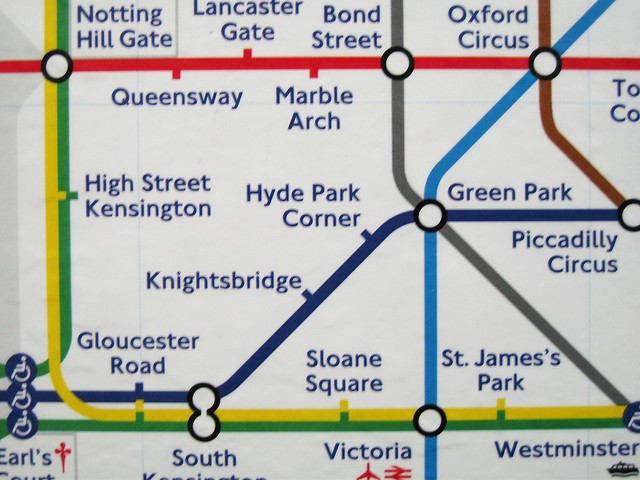
\includegraphics[scale=.50]{tubemap.jpg}
  \caption{\emph{London tube map}}
\end{subfigure}%
\begin{subfigure}{.5\textwidth}
  \centering
  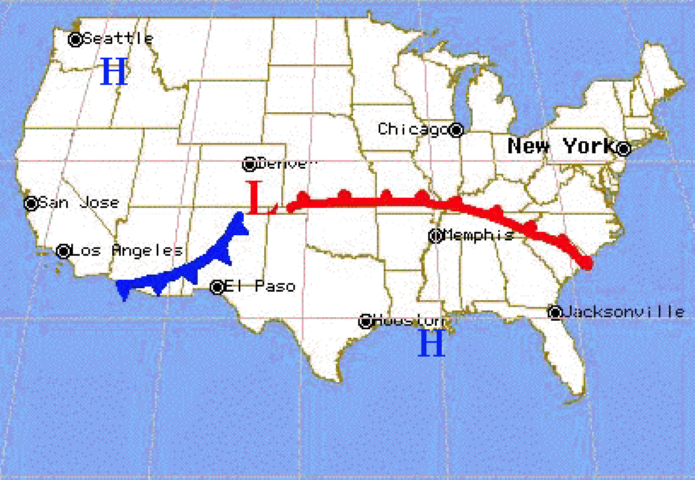
\includegraphics[scale=.25]{weather.png}
  \caption{\emph{Synoptic chart of weather in USA} }
\end{subfigure}
\begin{subfigure}{.5\textwidth}
  \centering
  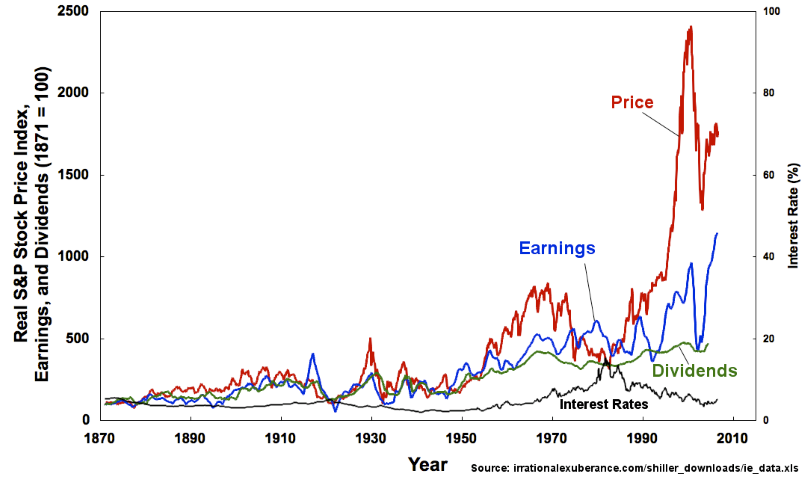
\includegraphics[scale=.25]{stockmarket.png}
  \caption{\emph{Plot of S\&P stock data} }
\end{subfigure}%
\begin{subfigure}{.5\textwidth}
  \centering
  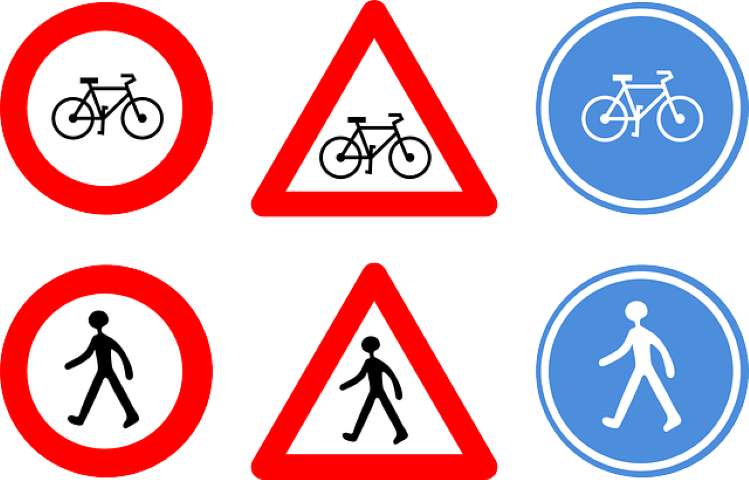
\includegraphics[scale=.25]{roadsigns.png}
  \caption{\emph{Bicycle and walking road signs} }
\end{subfigure}
\caption{\textit{Visualisation examples} (a)\citep{tubemap} (b)\citep{weather} (c)\citep{stockmarket}  (d)\citep{roadsigns}}
\label{fig:visualisations}
\end{figure}


\begin{figure}[!htb]
\centering

\begin{subfigure}{.5\textwidth}
  \centering
  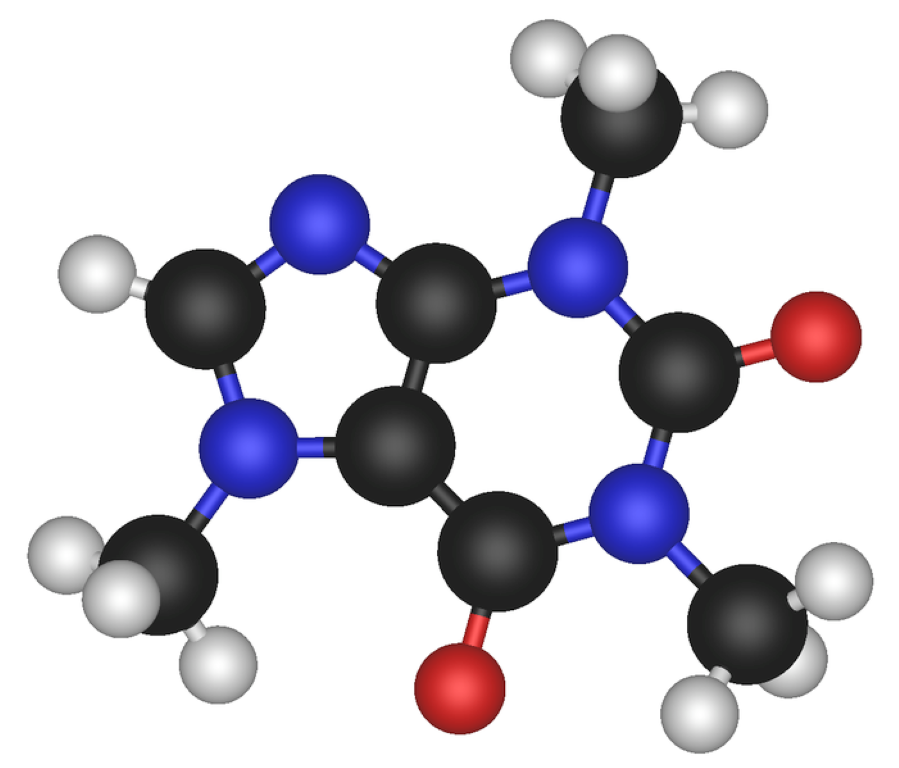
\includegraphics[scale=.20]{molecule.png}
  \caption{\emph{Caffeine molecule}}
\end{subfigure}%
\begin{subfigure}{.5\textwidth}
  \centering
  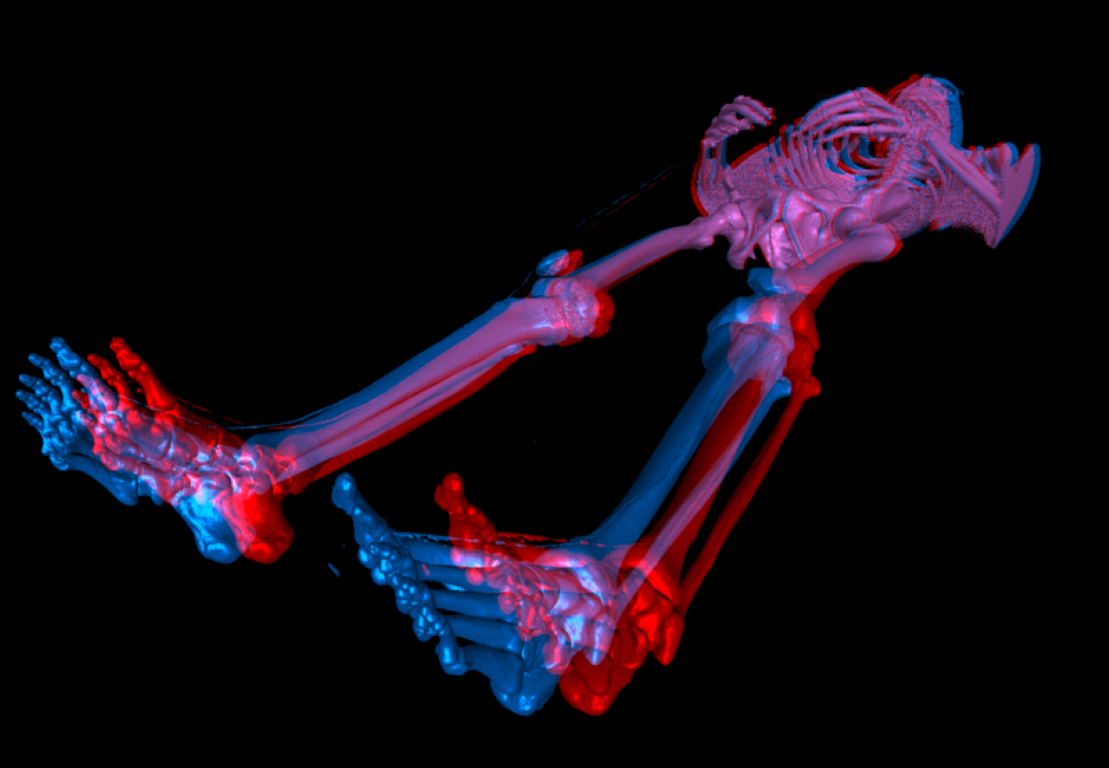
\includegraphics[scale=.20]{medicalvis.png}
  \caption{\emph{An anaglyph image of a human body} }
\end{subfigure}
\begin{subfigure}{.5\textwidth}
  \centering
  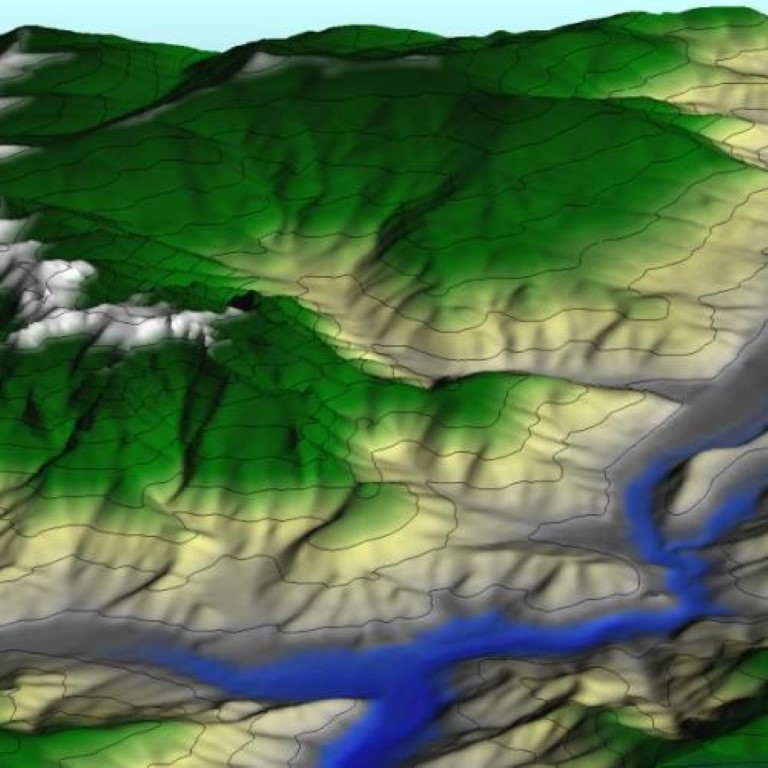
\includegraphics[scale=.20]{terrain.jpg}
  \caption{\emph{Terrain rendering} }
\end{subfigure}%
\begin{subfigure}{.5\textwidth}
  \centering
  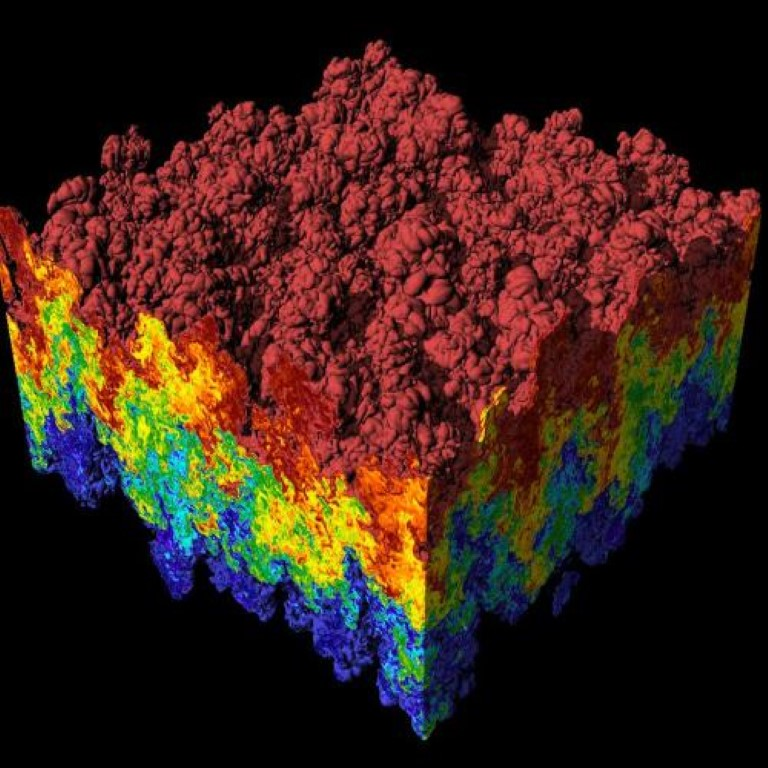
\includegraphics[scale=.20]{RayleighTaylor.jpg}
  \caption{\emph{Rayleigh-Taylor instability simulation} }
\end{subfigure}
\caption{\textit{Scientific visualisation} (a)\citep{molecule} (b)\citep{medicalvis} (c)\citep{rayleightaylor}  (d)\citep{terrain}}
\label{fig:scientificvisualisations}
\end{figure}

\subsection{Perception and cognition}

Cognition is a group of mental processes that includes attention, memory, learning, reasoning, and decision making. Perception is the processing of sensory information and is therefore a part of human cognition. Humans have a well developed sense of sight --- we perceive 75 percent of real world information visually. Visualisation is effective because it takes advantage of the brain's abilities, allowing us to gain insight more intuitively rather than through conscious thinking. 

\subsection{Visual search}

Visual search is a perceptual task requiring attention that involves the viewer actively scanning a visualisation or visual environment for a certain object or feature (the target) among other objects. There are various factors that can influence search performance. Basic attributes that can be considered to guide the deployment of attention (with a strong likelihood of supporting efficient search) are colour, motion, orientation and size \citep{wolfe04}.

\subsection{Graphical representation}

Visualisations are built from shapes and lines which have various properties such as size, length, width, height, volume, position, and colour. Additionally, these primitives can have dynamics that change over time, for example blinking or flashing. These visual properties are what is used to encode the information in a visualisation.

Visualisations can also consist of text (tag clouds introduced in \S\ref{sect:tagclouds} are an extreme example of this --- other visualisations may use text in passing, such as labelling an icon). Text can be manipulated to encode information through the use of typographical elements such as colour, font face and font styles.

\subsection{General techniques}

There are a great number of visualisation techniques that can be used. \cite{keim96} classified visualisation techniques according to their display mode:

\begin{enumerate}
\item \emph{Pixel-oriented techniques.} The arrangement of pixels, each dimension value mapped to a coloured pixel, grouped into adjacent areas. Pixel displays generally use one pixel per data value, so this technique can allow visualisation of large amounts of data depending on the display resolution. Appropriate arrangement of pixels can provide information on correlations and dependencies.

\item  \emph{Geometric projection techniques.} Geometrically transformed visualisations such as scatterplot matrices and parallel coordinates aim to show interesting properties of multi-dimensional datasets. In a parallel coordinate visualisation, dimensional spaces are mapped onto two display dimensions with axes that are parallel to each other. Each data element is depicted by connected line segments which intersect each of the axes (see Figure~\ref{fig:parallelcoordinates}). 

\begin{figure}[!htb]
  	 \centering
   	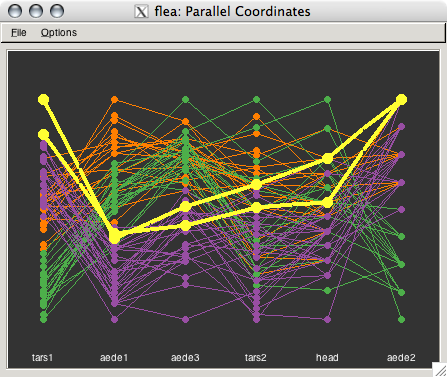
\includegraphics[scale=0.50]{parallelcoordinates.png}
  	\caption{\emph{Screenshot of GGobi, showing a parallel coordinate plot} \citep{parallelcoodinatesurl}}
	\label{fig:parallelcoordinates}
\end{figure}

\item  \emph{Icon-based techniques.} Iconic display methods map multi-dimensional data values to an icon by mapping the attribute values to features of the icon. An example of an iconic display is Chernoff faces \citep{chernoff73} as shown in Figure~\vref{fig:chernofffaces}. 

\begin{figure}[!htb]
  	 \centering
   	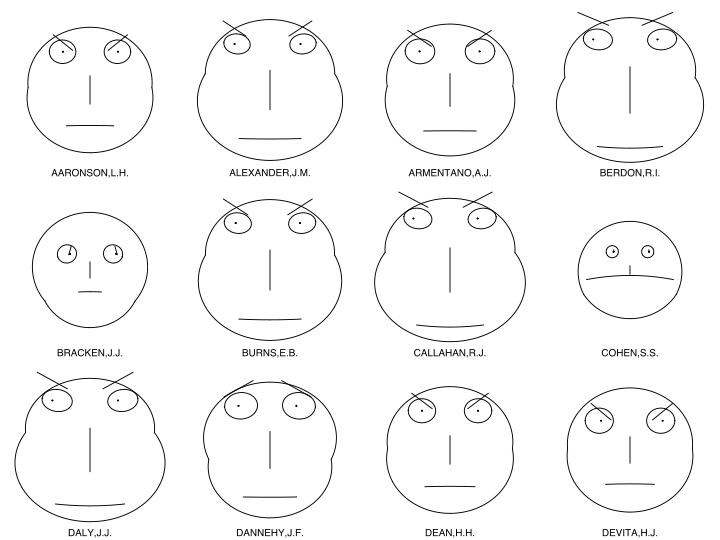
\includegraphics[scale=0.50]{chernofffaces.png}
  	\caption{\emph{Chernoff faces for evaluations of US judges} \citep{chernofffacesurl}}
	\label{fig:chernofffaces}
\end{figure}

\item  \emph{Hierarchical techniques.} Hierarchies are often drawn as node and edge diagrams, where a node is represented by a shape, and edges are represented by lines. Node and edge diagrams make inefficient use of space, with emptiness at the top left and right. Screen-filling techniques such as treemaps (see Figure~\vref{fig:treemap}) have been developed to fit large hierarchies onto the screen and use space more efficiently.

\item  \emph{Graph-based techniques.} Graph drawing facilitates understanding of relationships between objects. Graph-based techniques are used in trees, word graphs, and workflow diagrams. Specific layout algorithms are used to present large graphs.
\end{enumerate}

\subsection{Interaction techniques}

Interaction techniques are features that provide users with the ability to manipulate and interpret visualisations. There are a variety of ways that a user can interact and explore the data, for example:

\begin{description}
\item [Focus+Context] The underlying premise of Focus+Context is that the user may need both overview and detail information simultaneously. These two types of information can be combined within a single display, through interaction techniques such as fish-eye.

\item [Filtering] Uninteresting data elements can be filtered out. Dynamic queries can allow users to control the contents of the display, and focus on items of interest through elimination of other items.

\item [Zoom]  Items of interest may be zoomed in on. If users wish to know more about a particular area of the data, they can point to this location and click a mouse button until the required level of zooming is achieved.

\item [Brushing and linking] Brushing and linking allows multiple visualisations of a dataset to be be viewed simultaneously. Brushing of markers within the visualisations (such as in a scatterplot matrix) can then occur. The brushing and linking process involves selecting one element in a set of visualisations, brushing it with colour, then viewing the other linked visualisations to see the effect.

\end{description}

\section{Software visualisation}\label{sect:softvis}

As in information visualisation, in software engineering we want to explore abstract data to find trends and other interesting phenomena. We need help to comprehend and improve existing structures and build new ones. The examples given in Figures~\ref{fig:visualisations} and \ref{fig:scientificvisualisations} of information and scientific visualisation were all created with software. Given the success of visualisation in scientific and other research disciplines and the prolific examples of information visualisation and graphics in everyday life, computer generated visualisation and software engineering should be ideally suited. However, software visualisation is not widely practised or integrated into mainstream development environments.  An exception to this rule is UML diagrams, which are often used to create system diagrams of class structures and interactions (see Figure~\vref{fig:uml}). Even these diagrams, though, are often used for the development of new systems and may be largely ignored after the fact.

\begin{figure}[!htb]
   	\centering
  	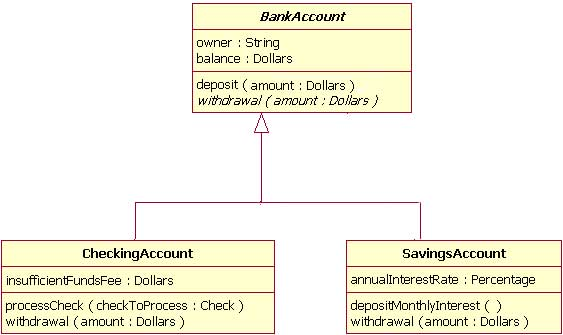
\includegraphics[scale=0.40]{uml.jpg}	
	\caption{\textit{UML Inheritance Diagram} \citep{uml}}
	\label{fig:uml}
\end{figure}

So what is the reason for the current lack of enthusiasm for software visualisation? \citet{reiss05} discusses this conundrum in his paper ``The paradox of Software Visualisation'', and outlines various possibilities which include reasons such as; lack of scaling to a suitable dataset size, interactive tools not providing answers to specific questions, low development workflow integration, lack of ease of use and high learning time, and neglect to adequately prove benefits. In the following sections, we describe the areas of software development where visualisations have been proposed, and introduce various devised techniques.

\subsection{What can we visualise?}\label{sect:whattovisualise}

Visualisation of software artefacts can help us in a number of areas, such as those detailed in Table~\vref{table:softwareartefacts}. A variety of approaches have been proposed for these areas.

\begin{table*}
\centering
\caption{\textit{Visualisation of Software Artefacts}}
\begin{tabular}{|p{6cm}|p{6cm}|} \hline
\textbf{Type}&\textbf{Area}\\ \hline
Quality assurance & metrics\par code smells\par heuristics \\ \hline
Process management & story/task management\par time allocation and management\par anomaly/issue detection\par project trends\par user achievement\par production support \\ \hline
Architecture & algorithms and control flow\par relationships and hierarchies\par interactions\par \\ \hline
Software evolution & source code repositories\par metrics\par structures \\ \hline
Runtime data & debugging\par memory management \\
\hline\end{tabular}
\label{table:softwareartefacts}
\end{table*}

\subsection{Quality assurance}\label{sect:qualityassurance}
 
Visualisation of software quality metric data often involves using a selection of multi-variate data visualisation techniques such as histograms, scatterplots or parallel coordinates. Kiviat charts (star glyphs) are also a commonly used technique for displaying multi-dimensional data.

Various 3D visualisations based on real-world metaphors like cities and landscapes have been developed. These have been applied in both software quality and architectural areas \citep[such as][]{irwin03, alam07} where metaphors such as 3D virtual worlds and building blocks have been explored.

It is possible to create ambient visualisations using alternate senses such as sound, odour, or vibration. \citet{murphyhill10} proposed a novel smell detector called Stench Blossom, that provided an interactive ambient visualisation designed to give programmers a high-level overview of the smells in their code. This and other visualisations of code smells such as jCosmo \citep{emden02} have been integrated in the development environment via a plugin.

\subsection{Process management}

Agile methodologies, used popularly in software project management, are inherently visual. Board views (used for story and task management) and burndown charts (time management, team status progression) are used in many agile teams. Also widely used are Gantt charts (a type of bar chart), which are visualisations incorporated into project management software illustrating a project schedule. 

\subsection{Architecture}

Algorithm visualisations for structured programming may be generated with graphical notations Nassi\textemdash Shneiderman diagrams (structograms). Nested boxes are used to represent simple statements and program control flow. Control flow graphs, first introduced by Frances E. Allen \citep{allen70}, show all paths that might be traversed through a program during its execution. These graphs are used in compiler optimisation and static program analysis tools.

Created by Booch, Rumbaugh and Jacobsen, Unified Modelling Language (UML) \citep{umlomg} is a popular and widely used set of graphical notations used to display relationships, interaction models and hierarchies in software. The set is comprised of a large number of diagrams including class/object models, use cases, behaviour and interaction diagrams, implementation diagrams and model management. These diagrams are most frequently used to visualise architectural elements of software.

Created by Ben Shneiderman in the nineties \citep{shneiderman09}, treemaps can show hierarchical data such as that found in software architecture, through the use of nested rectangles (see Figure~\vref{fig:treemap}).

\begin{figure} [!htb]
  	 \centering
   	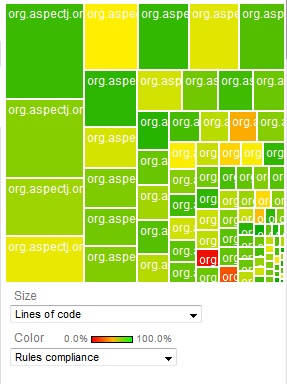
\includegraphics[width=60mm]{treemap.png}
  	\caption{\textit{Aspectj Treemap (created by the Sonar Software Analysis Platform)}}
	\label{fig:treemap}
\end{figure}

\subsection{Software evolution}

Visualisations of source code version histories are produced to analyse the evolution of a software system over time. This can reveal commonalities and irregularities in the development process. An example of this kind of visualisation is a `revision tower' \citep{taylor02} which allows people to see active areas of a project, how often changes are made, and how work is shared out.

Some tools produce visualisations of software metrics over time in order to provide a useful picture of software quality trends. One such example of this is the `SeeSoft system'\citep{eick92} which produces a space-filling visualisation for software metrics that are related to individual lines of code. Metrics such as code age can be viewed colour-coded, so that it is possible to see what parts of the system have recently been touched.

\subsection{Runtime data}

Dynamically generated visualisations to assist the debugging of runtime data are sometimes included as plugins in the development environment, such as the Eclipse Memory Analyser (MAT)\footnote{\url{http://www.eclipse.org/mat/}}. These tools may use a collection of visualisation techniques such as histograms, pie-charts and line graphs to illustrate measurements.

\section{Tag clouds}\label{sect:tagclouds}

Tag clouds are a common example of information visualisation found on the World Wide Web and are used to embody text --- words, two-word phrases and symbols. These items are grouped together to form a visual representation of the data.  Each element of the visualisation is referred to as a tag --- this may be website keywords which are hyperlinked to related resources. The frequency of a word (and therefore assumed importance) is highlighted by the font size or colour.  This makes the most important and prominent keywords easy to quickly identify as well as showing the relative importance of keywords. They can be displayed in a variety of layouts, most commonly alphabetically (see Figure~\vref{fig:tagcrowd} for a typical example).

\begin{figure}[htb]
   \centering
   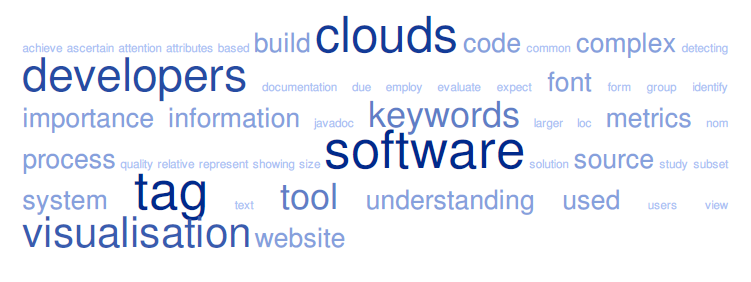
\includegraphics[width=140mm]{tagcrowd.png}
  \caption{\emph{Tag cloud created by TagCrowd}}
  \label{fig:tagcrowd}
\end{figure}

An early example of a weighted list of keywords can be found in Douglas Coupland's 1995 novel Microserfs. In this novel, a computer algorithm selects random phrases from an electronic diary creating a set of ``subconcious files''. In 2002 Jim Flanagan created a Perl module (Search Referral Zeitgeist), which generated a graphic of website referrers. Based on this implementation, photosharing site Flickr\footnote{\url{http://www.flickr.com}}, founded in 2004, created a ``tag cloud'' visualisation showing tag popularity through font size. Tag clouds then started appearing as a navigation aid on Web 2.0 websites such as Del.iocio.us\footnote{Now known as \url{http://www.delicious.com/}}.

The tag cloud was further adapted in 2006 by TagCrowd\footnote{\url{http://tagcrowd.com/}} for visualising word frequency in text, and then popularised by Wordle\footnote{\url{http://wordle.net/}} \citep{feinberg10}. Wordle showed tag clouds had the ability to be aesthetically pleasing (see Figure~\ref{fig:wordle}).

\begin{figure}[!htb]
   	\centering
   	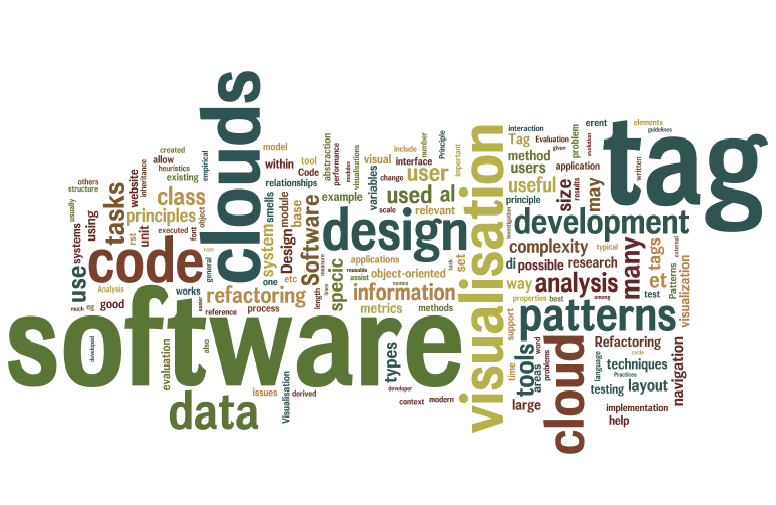
\includegraphics[width=140mm]{thesistagcloud.png}
  	\caption{\emph{Tag cloud created by Wordle}}
	\label{fig:wordle}	
\end{figure}

\subsection{Why tag clouds?}\label{sect:whytagclouds}

Tag clouds initially appear simple. This, along with high exposure online, makes them potentially more accessible to users than visualisations such as treemaps. This apparent simplicity may positively effect ease of use and learning ability, which were identified as important factors to visualisation takeup in the software engineering industry \citep{reiss05}. Another potential benefit of tag clouds is that they are reportedly perceived by some users to be visually interesting, appealing or otherwise aesthetically pleasing \citep{hearst08}. Some studies \citep[such as][]{kuo07} have also reported a high level of user satisfaction using them. 

In tag cloud visualisation, text labels are an intrinsic part of the visual encoding. This is particularly beneficial for software engineering datasets where textual labels are often used as identifiers.

Most current tag cloud implementations support limited interactivity. In order to effectively explore large datasets greater interactivity needs to be incorporated into the tag cloud visualisation interface, such as adding support for Shneiderman's visual information seeking mantra \citep{schneiderman96}.

\subsection{Tag clouds in software engineering}\label{sect:tagcloudsinsoftware}

In the software engineering domain, industry tools and academic research have not largely embraced tag clouds as a visualisation technique. There has been discussion of tag clouds for visualising relationships and structure \citep[such as][]{anslow08, bajracharya10, kurtz11} and also for source control evolution \citep[][]{kuhn12}. These examples show some interesting possibilities for inclusion of tag cloud based techniques in software engineering, but more extensive empirical evaluations are needed (of these papers only \citet{kurtz11} was included in the systematic mapping study detailed in Chapter~\ref{chap:strateval}, as it involved a usability evaluation). 

\subsection{Sourcecloud} 

In industry there are very few existing software engineering tools which utilise a tag cloud visualisation technique. Eclipse plugin Sourcecloud\footnote{\label{sourcecloud}\url{http://misto.ch/tag/eclipse/}} produces a Wordle-like visualisation of the text within a class, package or project with font size weighted by term frequency and colours assigned arbitrarily. The motivation behind this tool is to give an impression of how easy the code base is to understand by comparing proportions of domain-specific classname tags against core Java API classname tags.  We produced a visualisation of opensource project Aspectj\footnote{\label{aspectj}\url{http://www.eclipse.org/aspectj/}} (see Figure~\vref{fig:sourcecloud}). Some problems are apparent: the use of colour is a distracting factor (as it is not mapped to any variable), so some tags may appear more important than others without reason. An overview of all classes cannot be seen (due to a maximum word parameter), so words we are interested in may not be visible.

\begin{figure}[!htb]
   	\centering
  	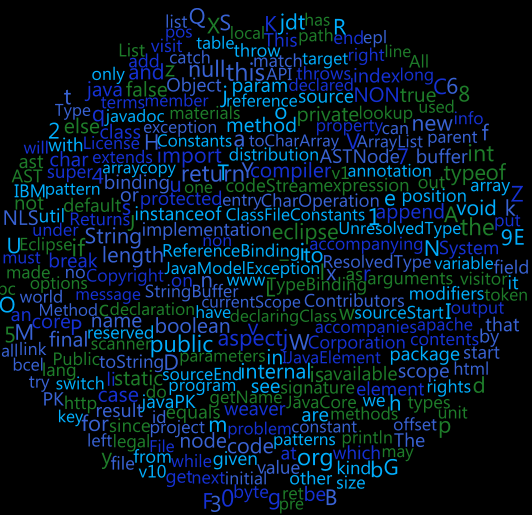
\includegraphics[scale=0.70]{sourcecloud.png}	
	\caption{\textit{AspectJ\textsuperscript{\ref{aspectj}} source code visualised with Sourcecloud\textsuperscript{\ref{sourcecloud}} }}
	\label{fig:sourcecloud}
\end{figure}

\subsection{Sonar platform} 

The Sonar Software Analysis Platform\footnote{\url{http://www.sonarsource.org/}}, which allows users to explore and visualise software metric data, comes bundled with a tag cloud component (see Figure~\vref{fig:aspectjsonar}). The tag font size is mapped to metric LOC (number of code lines for the class) and the tag colour is mapped to a rules compliance metric. The class name without the package can be problematic if different packages contained identically named classes. On the other hand, inclusion of the package name could dramatically increase the size of the cloud. The cloud produced is already a very large tag cloud, and may require scrolling. On the plus side, it is easy to quickly identify which classes contain a relatively large number of lines (CompletionEngine, CodeStream etc). The Sonar cloud tags are also used for navigation, and are hyperlinked through to pages showing individual metric data for the selected class. 

\begin{figure}[!htb]
   \centering
   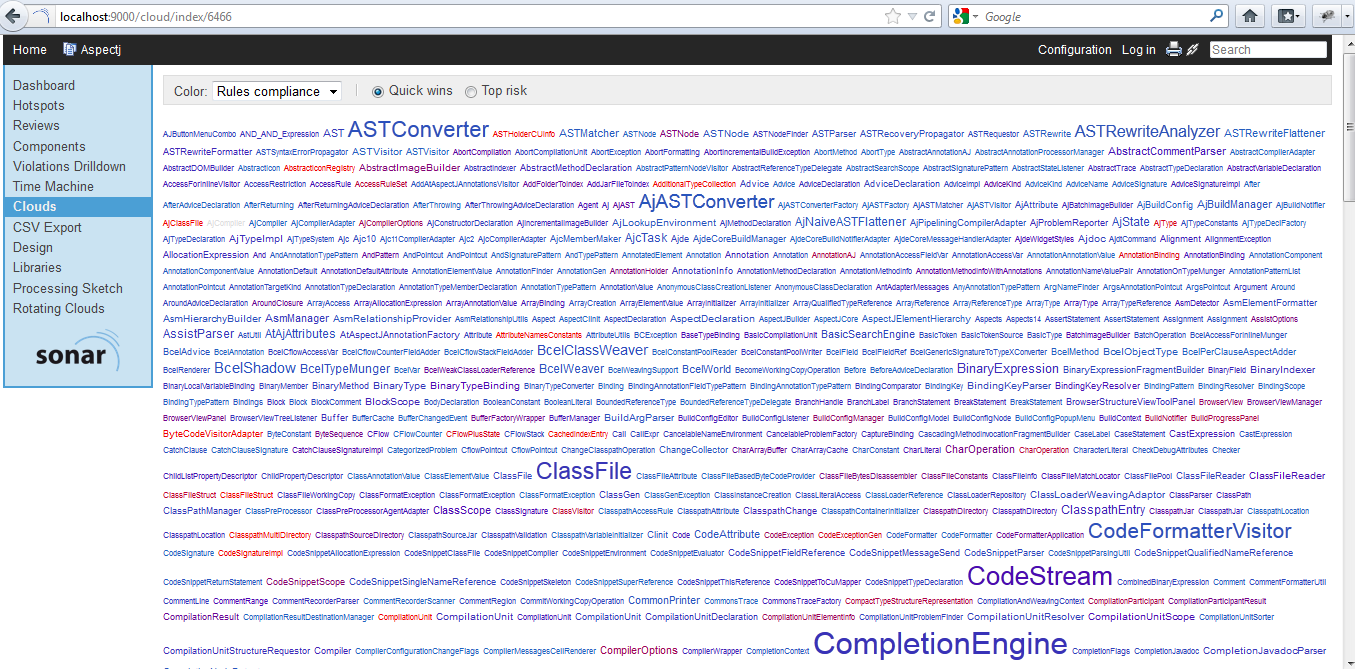
\includegraphics[scale=0.40]{sonarcloud.png}
  \caption{\textit{AspectJ\textsuperscript{\ref{aspectj}} visualised in Sonar}}
  \label{fig:aspectjsonar}
\end{figure}

\section{Summary and discussion} 

There is a comprehension problem in software development created by the huge size, constantly evolving nature and complex relationships. Modern ways to tackle aspects of scale and complexity include iterative development methodologies, automated unit testing and static or dynamic code analysis tools. Visualisation is a way to handle the reduced, but still overwhelming datasets we need to deal with in software engineering, and is considered useful in other domains (such as scientific research) as well as in general daily life. Despite a plethora of visualisation techniques suggested for the software domain, there remains a lack of widespread use of such techniques. 

Tag clouds are a highly recognisable visualisation of low-level complexity which deal primarily with text. Conventional implementations of tag clouds have limited interactivity which creates issues for data exploration. This research is focused on the evaluation of an interactive tag cloud visualisation tool. Can the tag cloud metaphor be extended to successfully visualise multi-variate data such as that found in software engineering? Both the Sourcecloud plugin and the Sonar platform visualisation show it is possible to apply the tag cloud technique directly to source code to identify and explore software quality metrics. Correspondingly, they also show the effectiveness of the technique relies on careful consideration given to various issues such as user perception of visual properties, and rich interactive features to allow data exploration.


% ------------------------------------------------------------------------


%%% Local Variables: 
%%% mode: latex
%%% TeX-master: "../thesis"
%%% End: 
